\documentclass[tikz,border=10pt]{standalone}

\usepackage{tikz}
\usetikzlibrary{arrows.meta, positioning}

\begin{document}

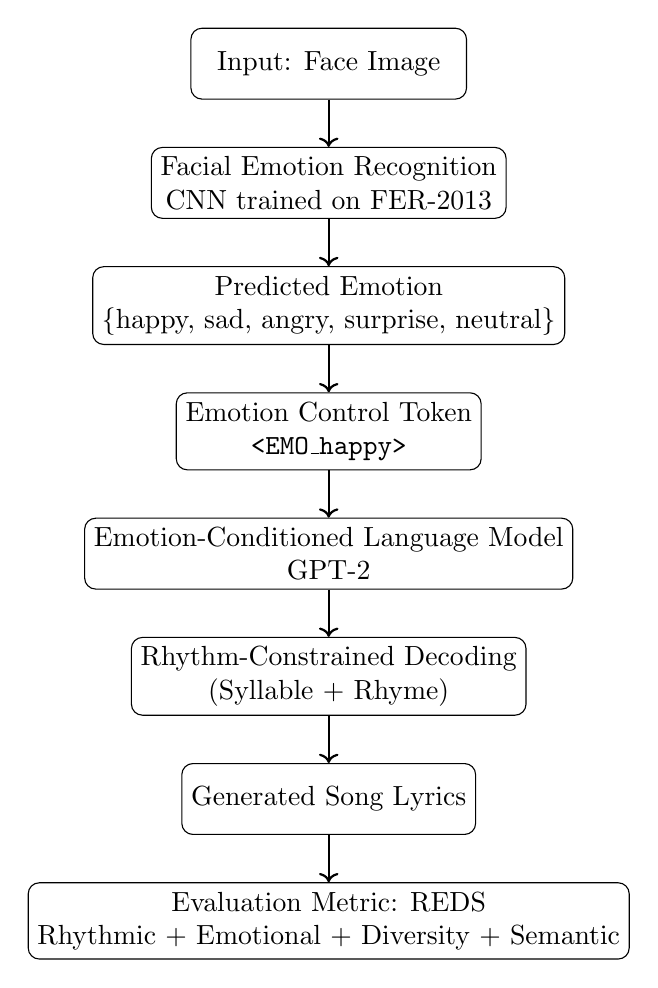
\begin{tikzpicture}[
node distance=0.6cm,
box/.style={draw, rectangle, rounded corners, align=center, minimum width=3.5cm, minimum height=0.9cm},
arrow/.style={->, thick}
]

\node[box] (input) {Input: Face Image};

\node[box, below=of input] (fer)
{Facial Emotion Recognition\\
CNN trained on FER-2013};

\node[box, below=of fer] (emotion)
{Predicted Emotion\\
\{happy, sad, angry, surprise, neutral\}};

\node[box, below=of emotion] (token)
{Emotion Control Token\\
\texttt{<EMO\_happy>}};

\node[box, below=of token] (gpt)
{Emotion-Conditioned Language Model\\
GPT-2};

\node[box, below=of gpt] (rhythm)
{Rhythm-Constrained Decoding\\
(Syllable + Rhyme)};

\node[box, below=of rhythm] (lyrics)
{Generated Song Lyrics};

\node[box, below=of lyrics] (reds)
{Evaluation Metric: REDS\\
Rhythmic + Emotional + Diversity + Semantic};

\draw[arrow] (input) -- (fer);
\draw[arrow] (fer) -- (emotion);
\draw[arrow] (emotion) -- (token);
\draw[arrow] (token) -- (gpt);
\draw[arrow] (gpt) -- (rhythm);
\draw[arrow] (rhythm) -- (lyrics);
\draw[arrow] (lyrics) -- (reds);

\end{tikzpicture}

\end{document}